\chapter{Klasifikacijska drevesa}
\label{ch:drevesa}

\newthought{Gradnja klasifikacijskih dreves je ena od najstarejših, a še vedno priljubljenih metod strojnega učenja.} Kakšna model je torej drevo?\marginnote{Klasifikacijska drevesa so bila izredno priljubljena metoda v zgodnjih dnev stronjega učenja, ko so jih neodvisno predlagali inženir Ross Quinlan (C4.5) in skupina statistikov (CART), vključno z očetom naključnih gozdov Leom Briemanom.}

Poglejmo si, kako je videti drevo na naših podatkih o genih. Za prikaz drevesa bomo uporabili gradnik \widget{Tree Viewer}.

\begin{figure}[h]
    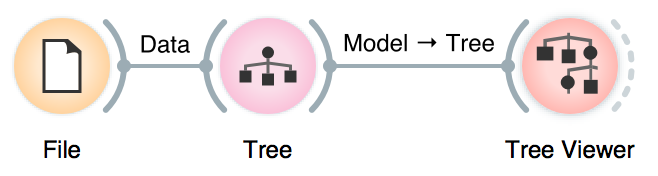
\includegraphics[width=0.8\linewidth]{workflow.png}
    \caption{$\;$}
\end{figure}

D\marginnote{Nekatera pravila izvedena s klasifikacijskim drevesom niso najbolj zanesljiva za majhne podatke. Koliko podatkov potrebujemo, da lahko pridemo do trdnejših zaključkov?}revesa beremo od zgoraj navzdol. Večina genov, 65 \%, je po funkciji ribosomov, kar označimo tudi v deblu drevesa. Spremenljivka, ki najlepše loči podatke na dva dela, tako da v njih prevlada en razred, je heat 20. Če je izraženost gena manjša od -0.16, gremo v levo vejo, sicer pa v desno. Poglejmo si levo vejo drevesa. 100 \% genov v tej veji je ribosomov; veja je povsem enotna. Na desni strani moramo deliti naprej in sicer po spremenljivki \textit{spo-mid}. Če je vrednost spo-mid manjša od 0.117, gremo levo, sicer desno. Obe končni veji sta izredno enotni. Drevo torej vzame najbolj informativne spremenljivke in po njih hierarhično razdeli drevo v podmnožice.

\begin{figure*}[h]
    \centering
    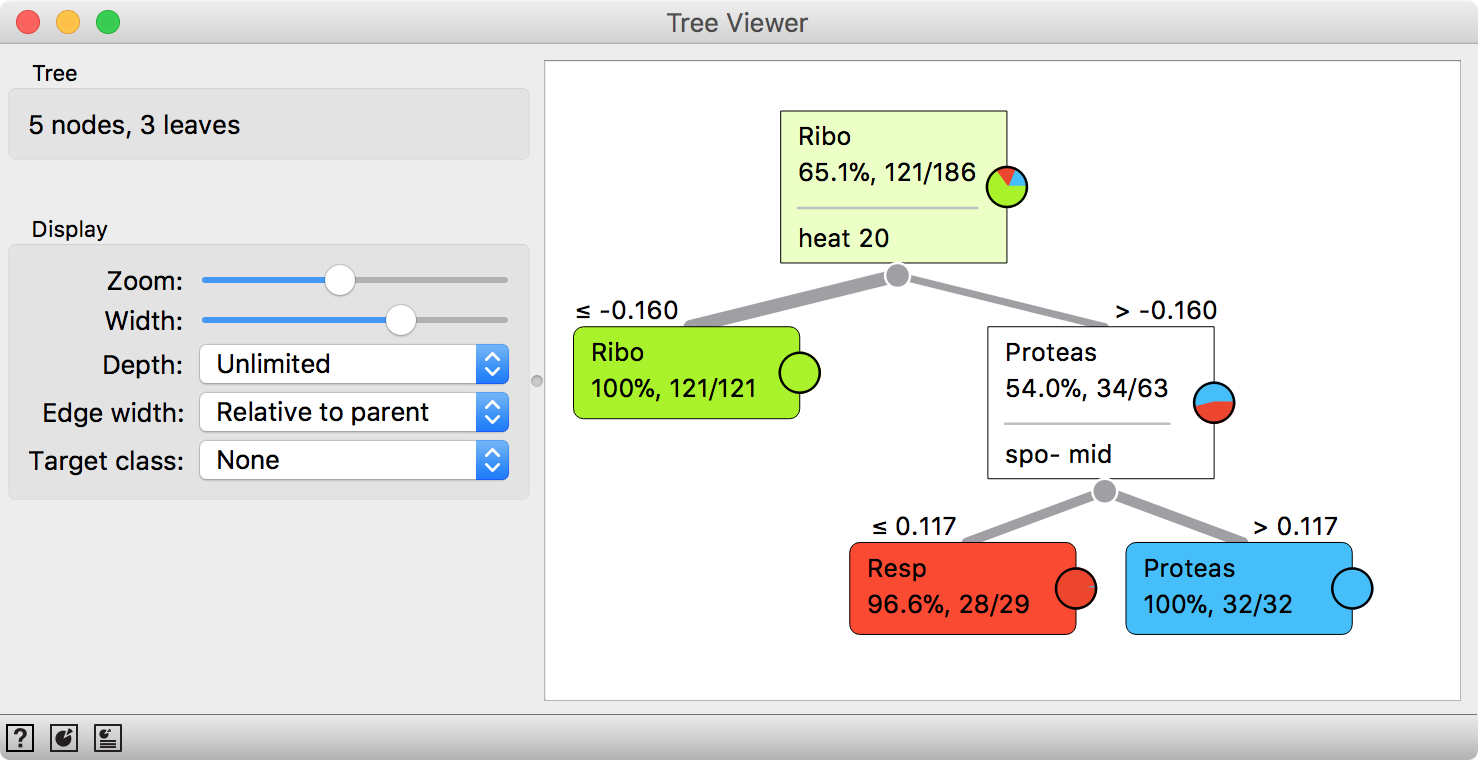
\includegraphics[width=0.8\linewidth]{tree.png}%
    \caption{$\;$}
\end{figure*}

Drevo se začne z najbolj uporabno spremenljivko. Kaj pa naj bi ta bila? To je spremenljivka, ki loči podatke v najbolj čisti podmnožici. Nato se podmnožice delijo naprej, po novih najboljših spremenljivkah, dokler vsi podatki v veji niso pripadniki enega razreda (močno rdeče, modre, zelene veje) oz. dokler ni v podmnožici premalo podatkov oz. dokler ne zmanjka uporabnih spremenljivk za deljenje.

Še vedno nismo bili čisto jasni glede ‘najbolj uporabne spremenljivke’. Mer kvalitete spremenljivk je veliko, temeljijo pa na tem, kako lepo ločijo razrede. Splošen koncept bomo prikazali z mero informacijskega prispevka. Mero lahko zračunamo z gradnikom \widget{Rank}, ki oceni kvaliteto spremenljivk in jih razvrsti po tem, koliko nam povedo o razredu. Informacijski prispevek lahko ocenimo na celotnih podatkih ali pa zgolj na eni od vej drevesa iz gradnika Tree Viewer.\marginnote{Na tem tečaju se ne bomo učili, kako izračunati informacijski prispevek. Na \href{stackoverflow.com}{stackoverflow.com} obstaja dobra razlaga koncepta s formulami in grafi (poguglajte).}

\begin{figure}[h]
    \centering
    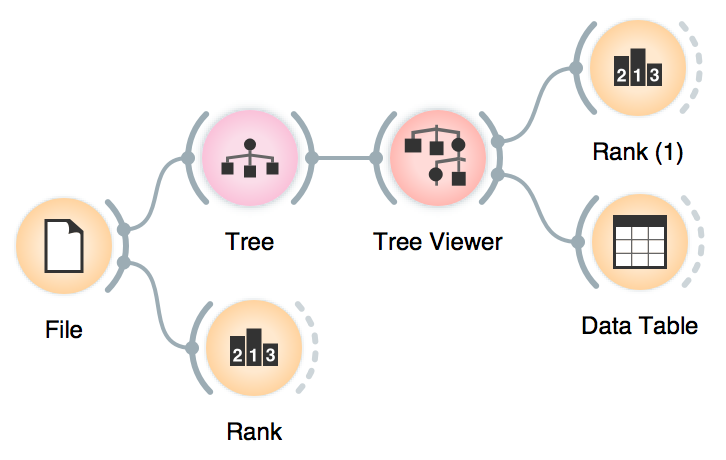
\includegraphics[width=0.8\linewidth]{workflow2.png}
    \caption{$\;$}
\end{figure}

Poleg informacijskega prispevka Rank prikaže še druge mere (npr. relativni informacijski prispevek in ginijev indeks), ki so velikokrat skladne med sabo in so bile izumljene za boljšo podporo kategoričnim spremenljivkam z več vrednostmi.

\begin{figure*}[h]
    \centering
    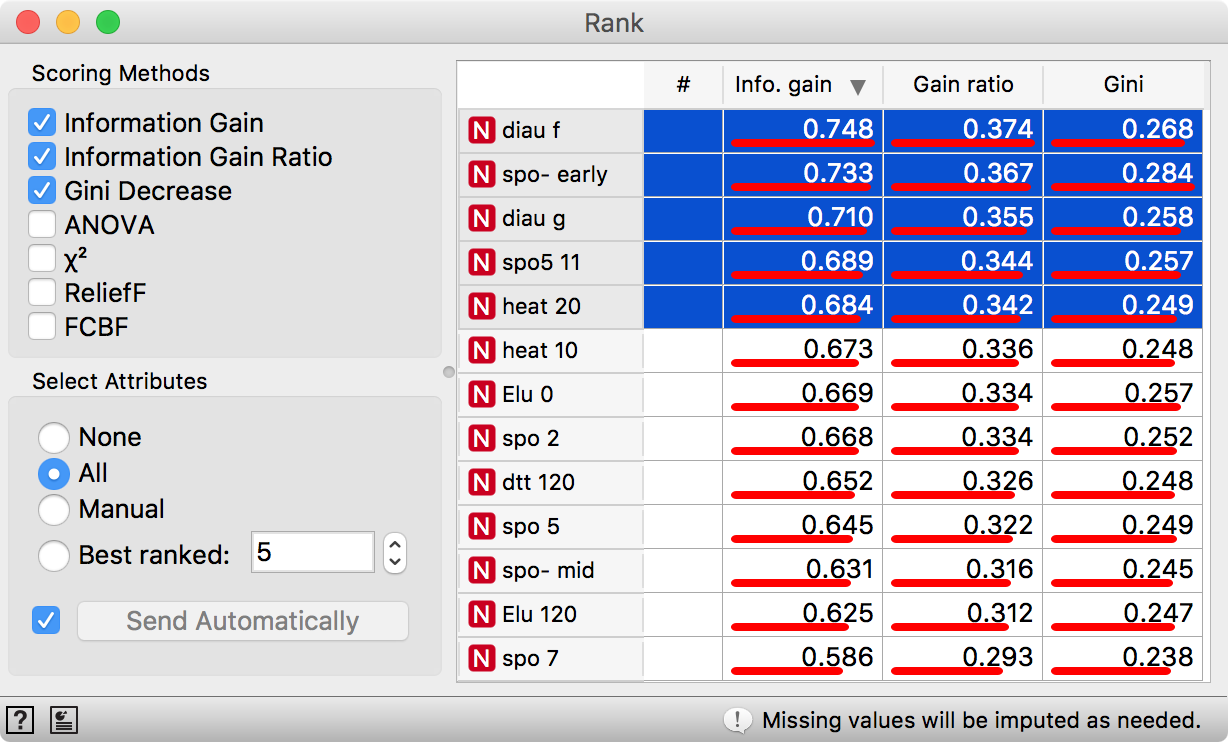
\includegraphics[width=0.8\linewidth]{rank.png}
    \caption{$\;$}
\end{figure*}
